\subsection{Acesso pela escotilha de dimensão grande}
Soluções que utilizem o acesso pela escotilha inferior, de dimensão maior,
apresentam as seguintes vantagens e desvantagens:

\textbf{Vantagens}:
\begin{itemize}
  \item Abertura maior para passagem de robôs pequenos montados ou um robô
  grande desmontado;
  \item Toda operação é realizada a seco;
  \item O acesso é livre;
  \item Este acesso já é usado pelos operadores para manutenção da turbina;
\end{itemize}

\textbf{Desvantagens}
\begin{itemize}
  \item Não é suficientemente grande para entrada de robôs de grande
  porte montados;
  \item Infraestrutura de transporte e complexa logística ao acesso por
  andaimes e talha;
  \item Dificuldade de movimentação e posicionamento do robô no aro câmara
  devido ao piso escorregadio e inclinado. Pode haver a necessidade de montagem
  de um plano horizontal; 
\end{itemize}

O acesso pela escotilha inferior apresenta, como todos os outros
acessos, um desafio logístico e o desafio comum do processo de metalização. O
acesso à escotilha é realizado por uma abertura de 80 mm de diâmetro e 4 m acima
do solo, logo os equipamentos são transportados por uma talha operada manualmente,
instalada dentro do aro câmara, em andaimes. O solo é escorregadio e, devido à
forma cilíndrica do aro câmara, curvilíneo e inclinado.

Dessa forma, as soluções foram focadas em robôs de médio porte, peso reduzido
devido ao transporte e às necessidades de movimentação e posicionamento do robô
(trajeto escotilha à pá), e modular, quando possível.

As soluções foram divididas em subseções de acordo com a fixação:
robôs móveis que se locomovem em trilhos, robôs escaladores e manipuladores
industriais com base fixa. 
%obs.:
%Colocar o robô entre as pás para aplicar revestimento de duas pás com uma
% instalação exige que o robô seja desmontado toda vez que a turbina for girada.
%Isso é ruim, pois após primeira aplicação a área fica de risco. Esta solução
%exige 5 movimentos no robô e 6 movimentos na turbina.

%A solução em que o robô fica atrás ou à frente exige que o robô seja
%movimentado apenas 2 vezes e a turbina fará 8 movimentos (duas voltas).

%TODO revisar todos os projetos sabendo as respostas
\subsubsection{Projeto de robôs em trilhos}\label{proj_rail}
 % attach a rail to the blade and move it manually
 
 % attach a rail one the nose and ground, 1D movement and move the blade to
A utlização de um manipulador robótico sobre trilhos satisfaz todos os
requisitos para a realização de um processo de inspeção e metalização utilizando a técnica HVOF. O desenvolvimento
de um sistema compacto para o transporte através do acesso pela escotilha
inferior e sua instalação no aro câmara da turbina são possíveis, pois as
dimensões do manipulador podem ser reduzidas por meio da
mobilidade extra proporcionada pela introdução do trilho.

No contexto da aplicação proposta, foram concebidas duas possibilidades para a
fixação do sistema de trilhos. A primeira solução consiste em um sistema
semelhante ao Roboturb, apresentado na seção \ref{sec::rail}. O sistema proposto
se trata de um manipulador robótico com fixação diretamente na própria pá da
turbina. O trilho deverá ser flexível para ser capaz de acompanhar a curvatura
da pá e possibilitar diversas opções de posicionamento. Como o material da pá
não possui alta permeabilidade magnética (Inox 420), a solução de fixação seria
por ventosas ativas e com material específico para suportar as grandes
variações de temperatura que a pá pode alcançar (temperatura ambiente a
$100^oC$ durante a metalização).

Uma abrangente pesquisa de robôs comerciais industriais de pequeno porte apontou
que há manipuladores com payload (entre 12 e 20 kg) e velocidade necessários,
sendo o LBR da Kuka o que possui melhor benefício peso/alcance, 30 Kg e 820 mm,
respectivamente. Para este manipulador, a metalização deverá ser
realizada em, pelo menos, quatro etapas com quatro trilhos diferentes e
customizados, e placas de sacrifício para evitar mau aplicação da metalização
durante as trocas de sentido na movimentação do robô.

A fixação de um trilho na pá apresenta diversas complexidades, como: a
necessidade de manualmente instalar/desinstalar o sistema trilho/robô oito vezes
em cada pá; o projeto do trilho customizado e flexível; e ventosas ativas
especiais que suportam variação de temperatura.

A alternativa para se evitar o contato com a pá consiste em um único trilho
retilíneo fixado por bases magnéticas no solo do aro câmara. Como o robô não
tem alcance de toda a pá, há, ainda, a necessidade de três posições verticais
diferentes. A pá pode ser processada em diagonal, e, neste caso, o manipulador
ficará responsável pela velocidade, posição e orientação do processo. Ou processada na
direção do trilho, e, neste caso, este ficará responsável pela velocidade e o
manipulador fará o controle de posição e orientação. Neste último, a troca de
sentido de movimento ocorrerá fora da pá, o que resulta na ausência de placas de
sacrifício. A figura~\ref{rail2} mostra o trilho externo à pá e com
processamento diagonal.

\begin{figure}[h!]
\centering
	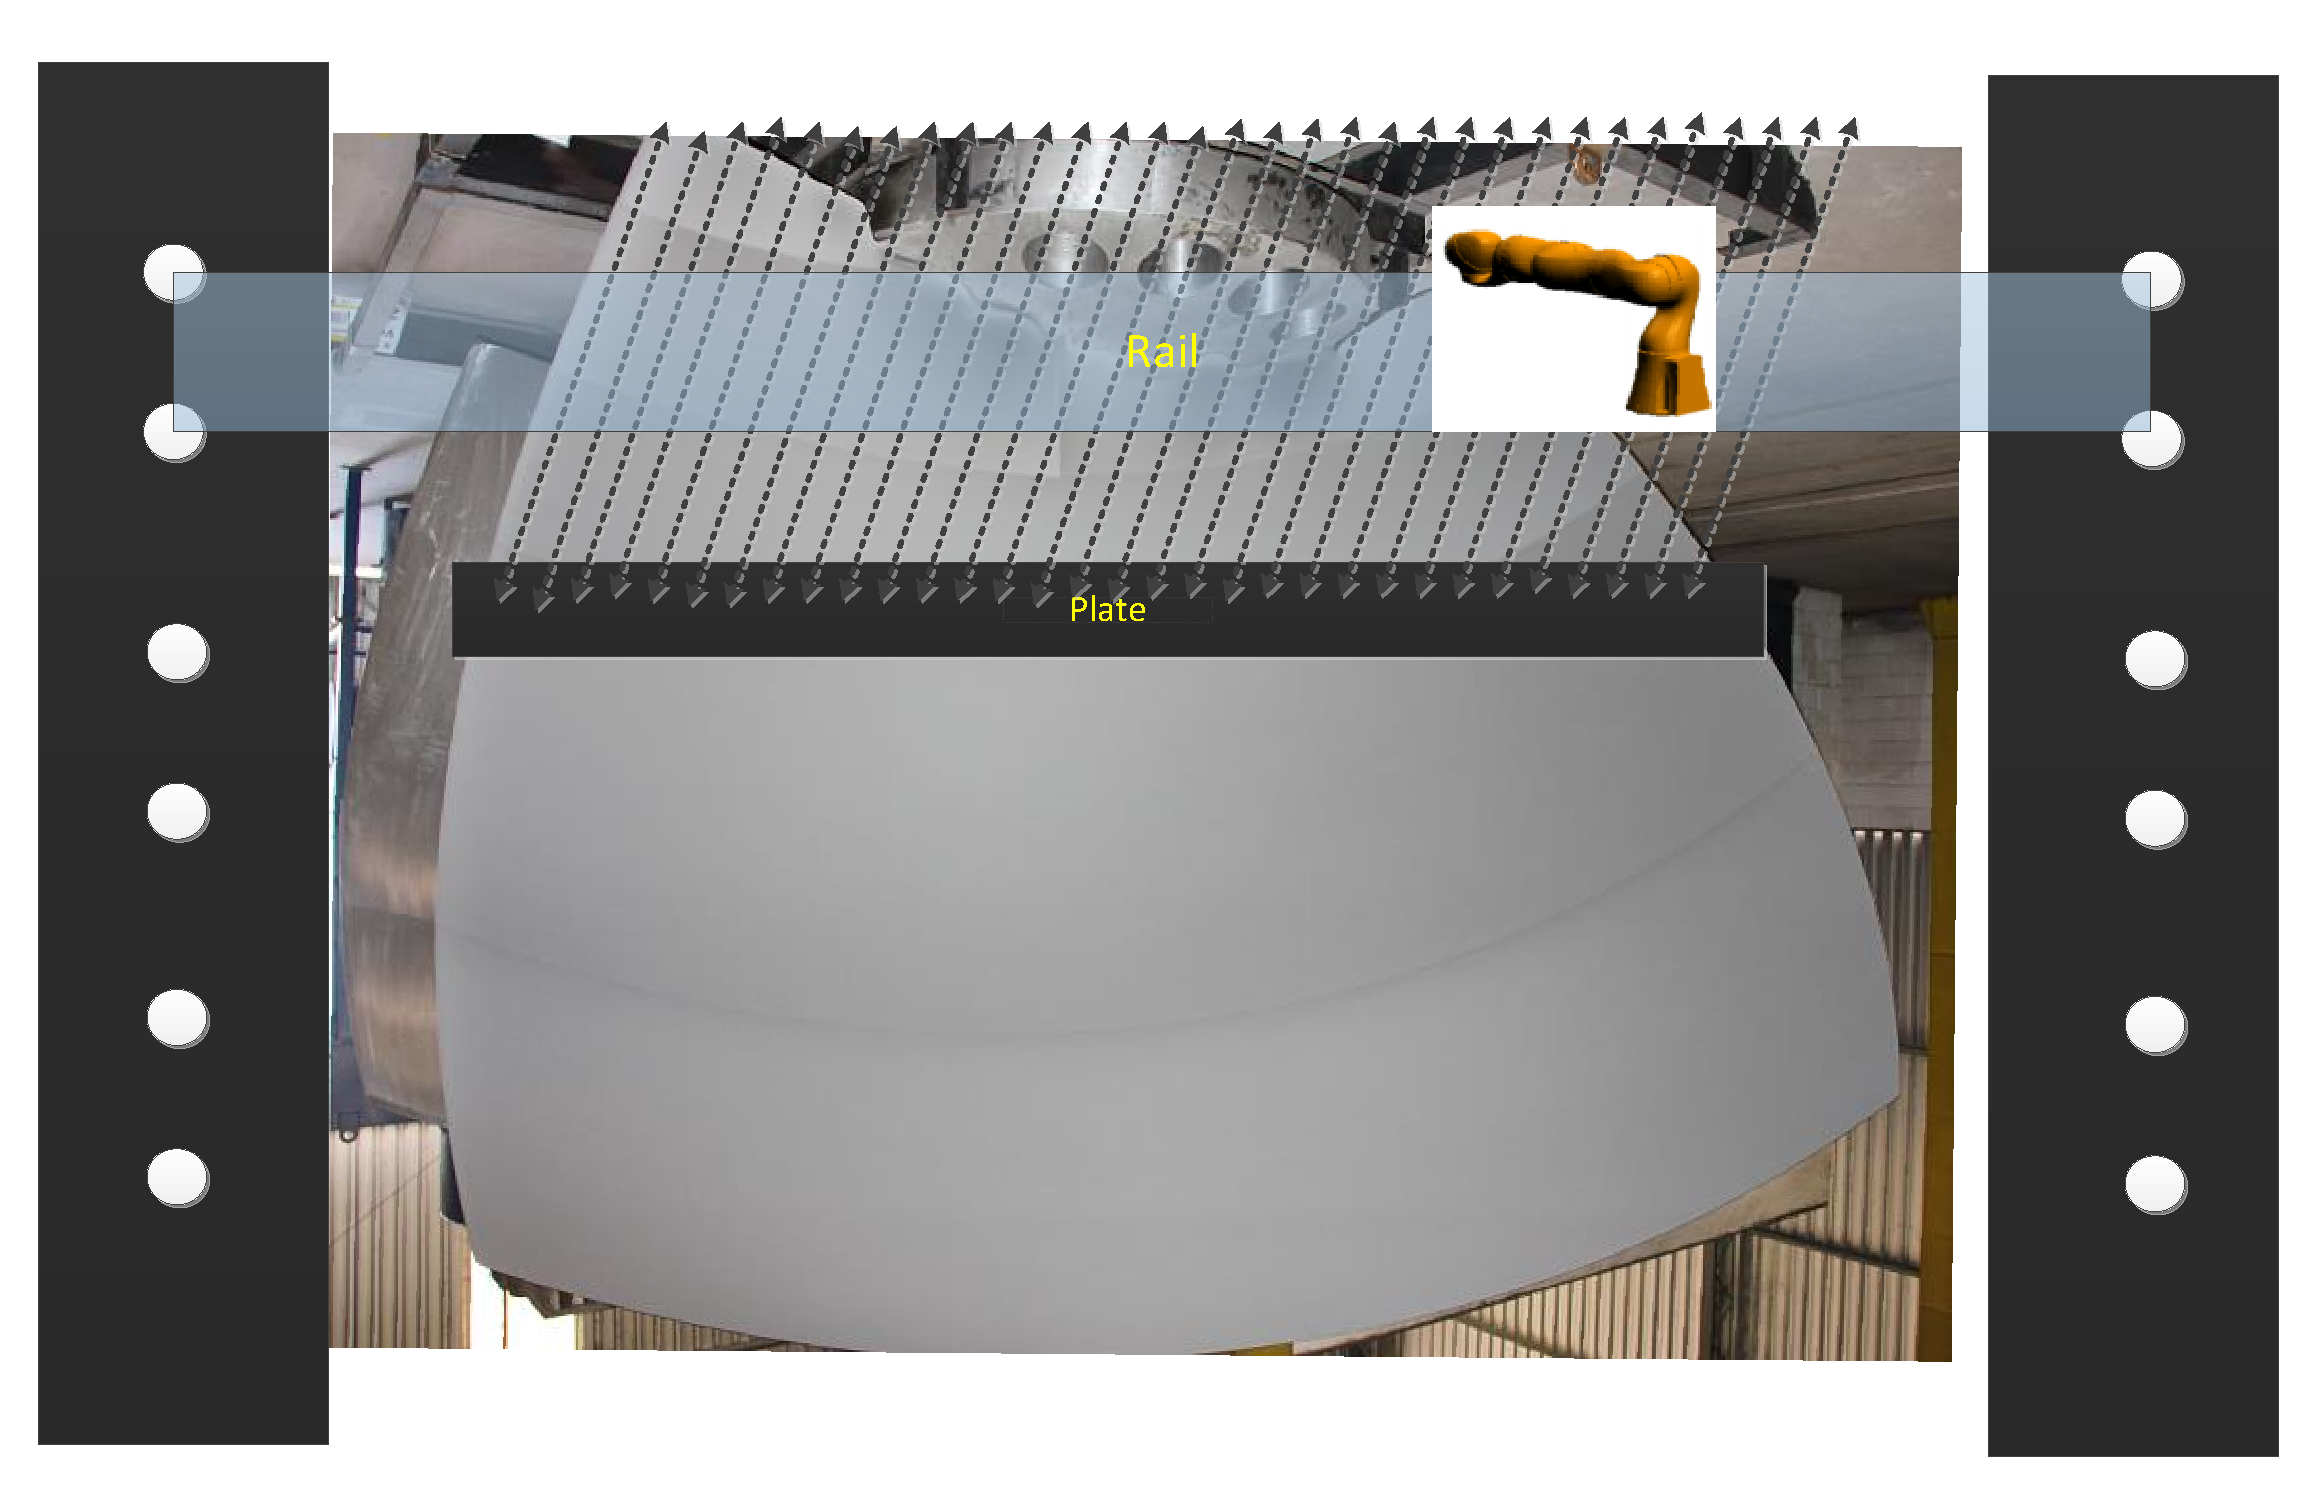
\includegraphics[width=\columnwidth]{figs/trilhos/rail2.pdf} 
	\caption{Trilho fora da pá com processamento em diagonal.}
	\label{rail2}
\end{figure}

Esse tipo de abordagem simplifica a movimentação do robô no
trilho, uma vez que o trilho seria totalmente reto, e possibilitaria a
metalização de um dos lados das quatro pás com uma única instalação de base.
Porém, mesmo nesta solução, a altura do trilho deverá ser ajustada três vezes para
cada lado de pá, e toda a estrutura deverá ser reinstalada no outro lado da
turbina para a realização do processo no outro lado das pás.

Em ambos os sistemas propostos, é necessária a implementação de um sistema de
localização do robô em relação à pá, tornando possível a geração de um
planejamento de trajetórias para o processo de metalização. O sistema de
localização pode ser concebido por sensores externos
ao robô (câmeras e outros), ou instalados no próprio manipulador/base.

\textbf{Conclusão da solução por robôs em trilhos}
A solução com trilho externo se mostrou vantajosa em comparação ao robô em
trilho customizado acoplado à pá, devido à complexidade e intervenções
manuais. Há a possibilidade de utilizar um manipulador industrial, tornando o
foco do projeto em processamento de sinais, mapeamento, localização e controle,
além da construção do trilho. Porém, a montagem da estrutura e a instalação de
todo o sistema atrás da pá podem ser custosas, sendo esta ainda uma solução
considerada complexa.
\subsection{Projeto de robôs escaladores}\label{proj_climbers}
% "scan" use succion-based mobile system (ICM climber) and place an arm on it.
% Is blade is above maximal curvature ?
% rail em movimento
Nesta subseção, consideram-se soluções para HVOF de pás de turbinas robôs
escaladores com fusão das tecnologias documentadas na
seção~\ref{sota}, subseção~\ref{sota_climbers}.

A solução mais completa, que mais atendia às especificações e possibilita
aperfeiçoamento 
\subsubsection{Projetos com manipuladores industriais fixos}\label{proj_manip}
Há diversos manipuladores robóticos industriais com as especificações
necessárias para a realização da tarefa de metalização por HVOF. As empresas
Fanuc, Motoman, ABB e KUKA fabricam manipuladores com dimensões compatíveis com o
acesso pela escotilha inferior e velocidade, precisão, e espaço de trabalho que
cumprem os requisitos para a execução do processo em todo um lado da pá, em uma
base fixa. Porém, há a necessidade de escolher a posição correta do manipulador
em relação à pá, a fim de maximizar a sua área de trabalho, no ambiente da
turbina, o que pode restringir os seus movimentos.
Como as pás podem ser giradas até um ângulo de $14.5^o$, são discutidas as ideias de posicionamento
do manipulador entre as pás, a fim de executar a operação em ambos os lados da
pá (um lado de cada pá), e o posicionamento fixo à frente da pá.

\textbf{Posicionamento entre pás}
A figura~\ref{fig::andaime} mostra o espaço entre as pás da turbina, dentro do
aro câmara. Um robô manipulador de médio porte pode ser fixado em uma base
magnética, na posição que se encontra a escada da figura~\ref{fig::andaime}.
Essa posição é vantajosa por possibilitar a execução da tarefa em duas pás
(frente de uma e verso da outra), sem desmontar ou fazer grandes alterações no
posicionamento da base do robô, diminuindo as intervenções e tempo de tarefa.

O estudo puramente geométrico demonstra que o alcance do manipulador robótico
para o processamento de ambos os lados das pás, considerando uma base fixa entre
as pás, deverá ser em torno de 5 metros. O manipulador industrial IRB5500,
desenvolvido pela ABB para pintura, possui 3 metros de alcance, porém 180 kg, o que já dificulta ou até impossibilita a
logística de movimentação e posicionamento in-situ. Não foi encontrado um robô
industrial com o alcance necessário e que tivesse as dimensões máximas da
escotilha inferior. 

A solução conceitual de posicionar um manipulador industrial entre as pás deve
avaliar, portanto, todas as configurações necessárias da base (orientações e
posições) para garantir que todo o espaço de trabalho do manipulador mais base
cubra os lados de ambas as pás. O número de configurações e o projeto
mecânico da base são extremamente necessários para a viabilização da solução,
uma vez que será possível avaliar as intervenções e complexidades. Bases
autônomas diminuem o número de intervenções e aumentam a precisção do sistema,
porém aumentam a complexidade, o custo devido ao número de sensores e atuadores
e o peso do sistema, prejudicando a logística.

\textbf{Posicionamento à frente da pá}
Posicionar de maneira fixa um manipulador com base magnética à frente da pá para
a metalização é uma solução natural, já que é semelhante à utilizada pela
empresa Rijeza atualmente. Um estudo puramente geométrico, utilizando as
dimensões da pá, mostra que o manipulador deve possuir alcance de 1.7 m e ser
posicionado a uma altura de 1.1 m em relação ao solo. Estudos de espaço de
trabalho, manipulabilidade e colisões devem ser realizados para confirmar o
estudo geométrico.

O posicionamento do sistema à frente da pá exige intervenções para rotação da
turbina e para o deslocamento do sistema para trás da pá. Em relação a um
sistema com base autônoma entre as pás, o processo parece mais custoso em
intervenções manuais e mais demorado, porém bem mais simples.

\textbf{Conclusão da solução com manipuladores industriais}
A utilização de manipuladores industriais é a mais simples dentre todas as soluções para o acesso pela escotilha inferior. Não há projeto mecânico
do manipulador, já que este será adquirido em um dos fabricantes citados. As
dificuldades mecânicas do projeto serão em relação à logística de posicionamento
e movimentação do robô dentro do aro câmara, e no desenvolvimento de uma base,
que pode ser autônoma. Além disso, o projeto fica responsável pelo controle do
manipulador, processamento de dados que envolvem o HVOF, planejamento de
trajetórias e UI.

Este projeto conceitual será uma das frentes para o estudo de viabilidade.
 
%% RIWEA-like rail on which the coating system
%  place blade horizontal and use wheels, against the blade's rim,to move a rail
  % along the blade's shape
  %  two-arm solution (or one arm + magnetic attachment point) to allow reaching
  % the top of the blade from the very bottom
\subsection{Robô Bipartido}

Esse conceito é uma cadeia de dois manipuladores conectados por um ponto de
apoio capaz de fixar-se à pá. O apoio serve como forma reduzir o torque
necessário nas juntas ao reduzir a alcance necessário para cada manipulador
individualmente.

Para facilitar futuras referências nesse texto, o braço robótico que se
apoia sobre o chão será chamado de primário, manipulador que parte dele de
secundário e o ponto de apoio entre eles, capaz de fixa-se à pá, será chamado de
fixador.

 A pistola de metalização presa ao manipulador secundário deve ter
alcance sobre toda a pá da turbina. Para isso existe uma gama de pontos
necessários onde o fixador deve ser posicionado. Com esse intuito o
manipulador primário da cadeia precisa ser projetado para ter uma região de
trabalho com um alcance total sobre esses pontos. Para tal, informações precisas
sobre o formato das pás são necessárias.

Para viabilizar a solução, é necessário verificar quais são as soluções
possíveis para gerar a aderencia do fixador sobre à pá. As tecnologias mais
difundidas são por força magnética e por diferença de pressão (ventosa).
As maiores preocupações com o relação a adesão são a capacidade de carga do
método e a resistência do \textit{coating}. As soluções por magnetismo e
por ventosa afetam de maneira diferente as camadas do material ao qual se
aderem. Enquanto o magnetismo atrai ativamente o material ao qual prentende
aderir, a ventosa apenas reduz a pressão do ar na região onde ela se fixa. Ambas
as soluções possuem versões ativas e passivas, assim como uma gama de opções com
relação à capacidade de suportar carga. Logo, para essas soluções, a carga
necessária a ser suportada, o magnetismo do material, a resistência à baixa
pressão do \textit{coating} e os efeitos da atração magnética, também, sobre o
\textit{coating} são perguntas que devem ser respondidas.

O braço secundário deve ser projetado para atingir os requerimentos de
posicionamento e velocidade da pistola de metalização, porém a região sob o
fixador, certamente, não estará disponivel para receber o revestimento. Assim, a
possibilidade, ou os requisitos necessários, de mover o fixador para uma região
da pá recém metalizada deve ser vista analisada antes do robô bipartido ser
considerado uma possibilidade.

\subsection{Robô Pendurado} 
